%!TEX root = ../../../thesis.tex

\label{Appendix:Measurements}


\section{Measurement scripts}

Energy consumption measurements were made using an Agilent E5270B
8-Slot Precision Measurement Mainframe, a Tektronix MSO 4054 Mixed
Signal Oscilloscope and a desktop PC. Operation of the E5270 was done
via GLIB interface using a USB connection and Agilent IO Libraries
Version 16.0.1458.0. From here the machine was interfaced using custom
Python scripts (appended) and PyVisa (available from \url{http://pyvisa.sourceforge.net/pyvisa/} ).

\subsection{E5270 Scripts}

Measurement of chip energy consumption was carried out using the following
measurement script. This script is written in Python and was executed
using PyLab from the Enthought Python bundle.

\verbatiminput{content/appendices/microprocessorPowerMeasurements/Microcontrollers/measDev.py}


\section{Measurement data}

It should be noted that the Freescale M9S08QG8 and the Microchip PIC16F1827
were unable to boot reliably into a low power state at 1.8V. To prevent
this from happening the chips were booted at 2.0V and lowered to 1.8V
to prevent the chips entering a state where current consumption was
in the hundreds of microamps range.


\subsection{Chips sleeping}

The following tables list the unprocessed current measurements for
a sweep of Vdd from 1.8V to 5.5V. Sweeps have been restricted to the
input voltage ranges as specified in each chips datasheet.

\begin{table}[htp]
\begin{centering}
\begin{tabular}{|r|r|r|r|r|r|}
\hline
Vdd  & Tiny13V  & Tiny25V  & 12F675  & 16F1827  & M9S08QG8\tabularnewline
\hline
1.80  & 3.41E-08  & 9.27E-08  & N/A  & 9.914E-07  & 3.82E-04 \tabularnewline
1.90  & 4.04E-08  & 9.30E-08  & N/A  & 1.008E-06  & 3.86E-04 \tabularnewline
2.00  & 4.73E-08  & 9.33E-08  & 4.497E-10  & 1.023E-06  & 4.88E-07 \tabularnewline
2.10  & 5.47E-08  & 9.36E-08  & 4.677E-10  & 1.038E-06  & 4.89E-07 \tabularnewline
2.20  & 6.26E-08  & 9.39E-08  & 4.797E-10  & 1.054E-06  & 4.91E-07 \tabularnewline
2.30  & 7.10E-08  & 9.42E-08  & 4.907E-10  & 1.068E-06  & 4.92E-07 \tabularnewline
2.40  & 7.99E-08  & 9.45E-08  & 5.057E-10  & 1.087E-06  & 4.94E-07 \tabularnewline
2.50  & 8.92E-08  & 9.47E-08  & 5.210E-10  & 1.102E-06  & 4.96E-07 \tabularnewline
2.60  & 9.90E-08  & 9.50E-08  & 5.347E-10  & 1.119E-06  & 4.99E-07 \tabularnewline
2.70  & 1.09E-07  & 9.53E-08  & 5.487E-10  & 1.137E-06  & 5.02E-07 \tabularnewline
2.80  & 1.20E-07  & 9.56E-08  & 5.610E-10  & 1.166E-06  & 5.05E-07 \tabularnewline
2.90  & 1.31E-07  & 9.59E-08  & 5.760E-10  & 1.195E-06  & 5.10E-07 \tabularnewline
3.00  & 1.42E-07  & 9.63E-08  & 5.903E-10  & 1.234E-06  & 5.15E-07 \tabularnewline
3.10  & 1.54E-07  & 9.66E-08  & 6.057E-10  & 1.290E-06  & 5.21E-07 \tabularnewline
3.20  & 1.67E-07  & 9.70E-08  & 6.217E-10  & 1.300E-06  & 5.28E-07 \tabularnewline
3.30  & 1.79E-07  & 9.74E-08  & 6.397E-10  & 1.301E-06  & 5.37E-07 \tabularnewline
3.40  & 1.92E-07  & 9.78E-08  & 6.590E-10  & 1.302E-06  & 5.47E-07 \tabularnewline
3.50  & 2.06E-07  & 9.82E-08  & 6.763E-10  & 1.301E-06  & 5.60E-07 \tabularnewline
3.60  & 2.20E-07  & 9.87E-08  & 6.970E-10  & 1.304E-06  & 5.75E-07 \tabularnewline
3.70  & 2.35E-07  & 9.93E-08  & 7.200E-10  & 1.307E-06  & N/A \tabularnewline
3.80  & 2.49E-07  & 1.00E-07  & 7.437E-10  & 1.309E-06  & N/A \tabularnewline
3.90  & 2.65E-07  & 1.01E-07  & 7.703E-10  & 1.311E-06  & N/A \tabularnewline
4.00  & 2.80E-07  & 1.02E-07  & 7.960E-10  & 1.312E-06  & N/A \tabularnewline
4.10  & 2.97E-07  & 1.03E-07  & 8.273E-10  & 1.317E-06  & N/A \tabularnewline
4.20  & 3.13E-07  & 1.04E-07  & 8.690E-10  & 1.319E-06  & N/A \tabularnewline
4.30  & 3.31E-07  & 1.05E-07  & 9.033E-10  & 1.330E-06  & N/A \tabularnewline
4.40  & 3.48E-07  & 1.07E-07  & 9.487E-10  & 1.334E-06  & N/A \tabularnewline
4.50  & 3.67E-07  & 1.09E-07  & 9.977E-10  & 1.342E-06  & N/A \tabularnewline
4.60  & 3.86E-07  & 1.11E-07  & 1.056E-09  & 1.351E-06  & N/A \tabularnewline
4.70  & 4.05E-07  & 1.13E-07  & 1.117E-09  & 1.360E-06  & N/A \tabularnewline
4.80  & 4.25E-07  & 1.16E-07  & 1.197E-09  & 1.373E-06  & N/A \tabularnewline
4.90  & 4.46E-07  & 1.19E-07  & 1.296E-09  & 1.385E-06  & N/A \tabularnewline
5.00  & 4.67E-07  & 1.23E-07  & 1.403E-09  & 1.401E-06  & N/A \tabularnewline
5.10  & 4.90E-07  & 1.27E-07  & 1.513E-09  & 1.422E-06  & N/A \tabularnewline
5.20  & 5.13E-07  & 1.32E-07  & 1.661E-09  & 1.445E-06  & N/A \tabularnewline
5.30  & 5.37E-07  & 1.38E-07  & 1.811E-09  & 1.469E-06  & N/A \tabularnewline
5.40  & 5.62E-07  & 1.45E-07  & 1.975E-09  & 1.497E-06  & N/A \tabularnewline
5.50  & 5.88E-07  & 1.53E-07  & 2.164E-09  & 1.529E-06  & N/A \tabularnewline
\hline
\end{tabular}
\par\end{centering}

\protect\caption{Raw sleep measurements (Vdd 1.8V -- 5.5V)}
\end{table}
\begin{figure}
\begin{centering}
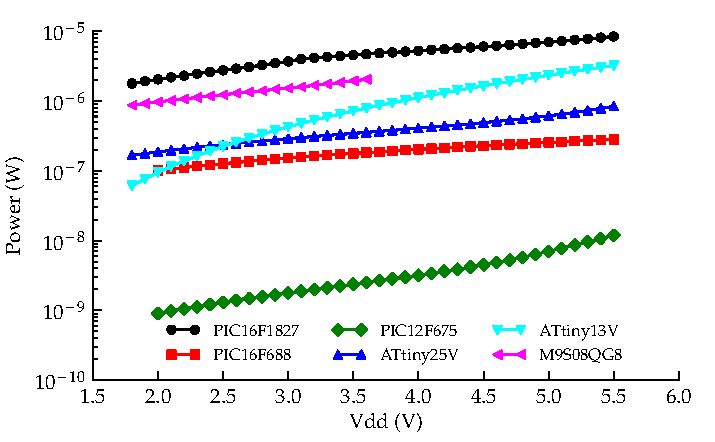
\includegraphics{content/appendices/microprocessorPowerMeasurements/graphics/Graph_All_Sleeping_Power}
\par\end{centering}

\protect\caption{\label{fig:All_SleepPower}Power usage of each microprocessor while
in sleep mode}


\end{figure}


Figure \ref{fig:All_Sleep_Current} shows the amount of current drawn
by each of the microprocessors in sleep mode. Similarly, figure \ref{fig:All_SleepPower}
shows the power consumption of each of the chips in sleep mode.


\subsection{Clocking}


\subsubsection*{ATtiny13V}

\begin{sidewaystable}
\begin{centering}
\begin{tabular}{|r|r|r|r|r|r|r|}
\hline
Vdd  & 9.6 MHz  & 4.8 MHz  & 1.2 MHz  & 600 kHz  & 128 kHz  & 16 kHz\tabularnewline
\hline
1.80  & N/A  & N/A  & 3.900E-04  & 2.148E-04  & 8.098E-05  & 5.393E-05 \tabularnewline
1.90  & N/A  & N/A  & 4.121E-04  & 2.258E-04  & 8.387E-05  & 5.499E-05 \tabularnewline
2.00  & N/A  & N/A  & 4.242E-04  & 2.329E-04  & 8.708E-05  & 5.608E-05 \tabularnewline
2.10  & N/A  & N/A  & 4.429E-04  & 2.421E-04  & 8.897E-05  & 5.721E-05 \tabularnewline
2.20  & N/A  & N/A  & 4.634E-04  & 2.523E-04  & 9.126E-05  & 5.839E-05 \tabularnewline
2.30  & N/A  & N/A  & 4.859E-04  & 2.632E-04  & 9.415E-05  & 5.964E-05 \tabularnewline
2.40  & N/A  & N/A  & 5.088E-04  & 2.748E-04  & 9.738E-05  & 6.099E-05 \tabularnewline
2.50  & N/A  & N/A  & 5.323E-04  & 2.865E-04  & 1.006E-04  & 6.214E-05 \tabularnewline
2.60  & N/A  & N/A  & 5.557E-04  & 2.984E-04  & 1.038E-04  & 6.396E-05 \tabularnewline
2.70  & 2.759E-03  & 1.664E-03  & 5.799E-04  & 3.108E-04  & 1.071E-04  & 6.560E-05 \tabularnewline
2.80  & 2.879E-03  & 1.742E-03  & 6.065E-04  & 3.235E-04  & 1.102E-04  & 6.743E-05 \tabularnewline
2.90  & 3.001E-03  & 1.834E-03  & 6.384E-04  & 3.366E-04  & 1.136E-04  & 6.926E-05 \tabularnewline
3.00  & 3.116E-03  & 1.945E-03  & 6.705E-04  & 3.540E-04  & 1.174E-04  & 7.100E-05 \tabularnewline
3.10  & 3.231E-03  & 2.022E-03  & 6.876E-04  & 3.582E-04  & 1.124E-04  & 6.809E-05 \tabularnewline
3.20  & 3.358E-03  & 2.109E-03  & 7.144E-04  & 3.710E-04  & 1.150E-04  & 6.878E-05 \tabularnewline
3.30  & 3.486E-03  & 2.199E-03  & 7.421E-04  & 3.843E-04  & 1.175E-04  & 6.996E-05 \tabularnewline
3.40  & 3.619E-03  & 2.295E-03  & 7.700E-04  & 3.979E-04  & 1.200E-04  & 7.115E-05 \tabularnewline
3.50  & 3.757E-03  & 2.394E-03  & 7.976E-04  & 4.114E-04  & 1.226E-04  & 7.235E-05 \tabularnewline
3.60  & 3.905E-03  & 2.491E-03  & 8.269E-04  & 4.251E-04  & 1.250E-04  & 7.354E-05 \tabularnewline
\hline
\end{tabular}
\par\end{centering}

\protect\caption{Atmel ATtiny13V clocking current (Vdd 1.8V -- 3.6V).}


\end{sidewaystable}
\begin{sidewaystable}
\begin{centering}
\begin{tabular}{|r|r|r|r|r|r|r|}
\hline
Vdd  & 9.6 MHz  & 4.8 MHz  & 1.2 MHz  & 600 kHz  & 128 kHz  & 16 kHz\tabularnewline
\hline
3.70  & 4.046E-03  & 2.580E-03  & 8.555E-04  & 4.392E-04  & 1.275E-04  & 7.471E-05 \tabularnewline
3.80  & 4.185E-03  & 2.661E-03  & 8.854E-04  & 4.535E-04  & 1.298E-04  & 7.706E-05 \tabularnewline
3.90  & 4.322E-03  & 2.740E-03  & 9.156E-04  & 4.685E-04  & 1.321E-04  & 7.701E-05 \tabularnewline
4.00  & 4.464E-03  & 2.822E-03  & 9.467E-04  & 4.834E-04  & 1.343E-04  & 7.814E-05 \tabularnewline
4.10  & 4.606E-03  & 2.900E-03  & 9.780E-04  & 4.990E-04  & 1.365E-04  & 7.929E-05 \tabularnewline
4.20  & 4.753E-03  & 2.932E-03  & 1.010E-03  & 5.152E-04  & 1.386E-04  & 8.045E-05 \tabularnewline
4.30  & 4.901E-03  & 2.991E-03  & 1.043E-03  & 5.313E-04  & 1.406E-04  & 8.163E-05 \tabularnewline
4.40  & 5.061E-03  & 3.001E-03  & 1.077E-03  & 5.491E-04  & 1.425E-04  & 8.283E-05 \tabularnewline
4.50  & 5.219E-03  & 2.987E-03  & 1.110E-03  & 5.655E-04  & 1.444E-04  & 8.406E-05 \tabularnewline
4.60  & 5.389E-03  & 3.073E-03  & 1.144E-03  & 5.833E-04  & 1.462E-04  & 8.531E-05 \tabularnewline
4.70  & 5.547E-03  & 3.162E-03  & 1.178E-03  & 6.002E-04  & 1.480E-04  & 8.661E-05 \tabularnewline
4.80  & 5.710E-03  & 3.257E-03  & 1.213E-03  & 6.216E-04  & 1.498E-04  & 8.795E-05 \tabularnewline
4.90  & 5.872E-03  & 3.348E-03  & 1.248E-03  & 6.395E-04  & 1.502E-04  & 8.932E-05 \tabularnewline
5.00  & 6.046E-03  & 3.443E-03  & 1.285E-03  & 6.567E-04  & 1.484E-04  & 9.072E-05 \tabularnewline
5.10  & 6.228E-03  & 3.548E-03  & 1.320E-03  & 6.746E-04  & 1.470E-04  & 9.213E-05 \tabularnewline
5.20  & 6.391E-03  & 3.647E-03  & 1.357E-03  & 6.940E-04  & 1.465E-04  & 9.346E-05 \tabularnewline
5.30  & 6.575E-03  & 3.753E-03  & 1.394E-03  & 7.134E-04  & 1.469E-04  & 9.482E-05 \tabularnewline
5.40  & 6.753E-03  & 3.857E-03  & 1.434E-03  & 7.331E-04  & 1.485E-04  & 9.640E-05 \tabularnewline
5.50  & 6.955E-03  & 3.970E-03  & 1.471E-03  & 7.526E-04  & 1.506E-04  & 9.818E-05 \tabularnewline
\hline
\end{tabular}
\par\end{centering}

\protect\caption{Atmel ATtiny13V clocking current (Vdd 3.7V -- 5.5V).}


\end{sidewaystable}
\begin{figure}
\begin{centering}
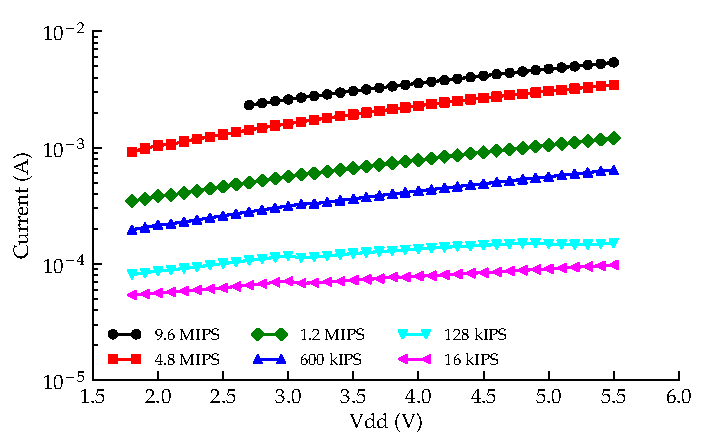
\includegraphics{content/appendices/microprocessorPowerMeasurements/graphics/Graph_ATtiny13V_Clock_Current}
\par\end{centering}

\protect\caption{
\label{fig:ATtiny13VClkCurrent}Current consumption of the Atmel ATtiny13V
while clocking
}


\end{figure}
\begin{figure}
\begin{centering}
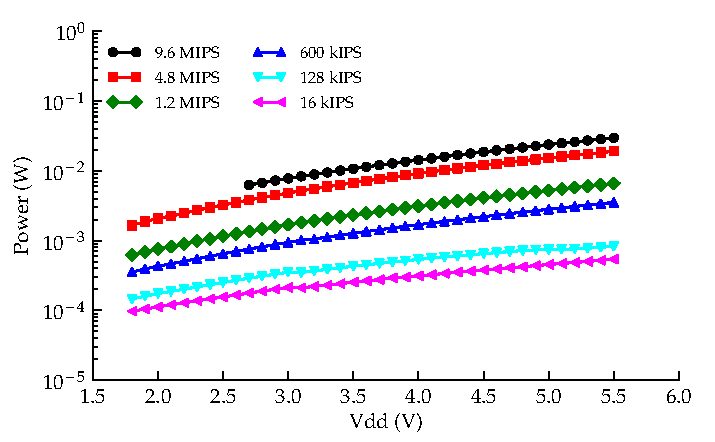
\includegraphics{content/appendices/microprocessorPowerMeasurements/graphics/Graph_ATtiny13V_Clock_Power}
\par\end{centering}

\protect\caption{
\label{fig:ATtiny13VClkPower}Power consumption of the Atmel ATtiny13V
while clocking
}
\end{figure}
\begin{figure}
\begin{centering}
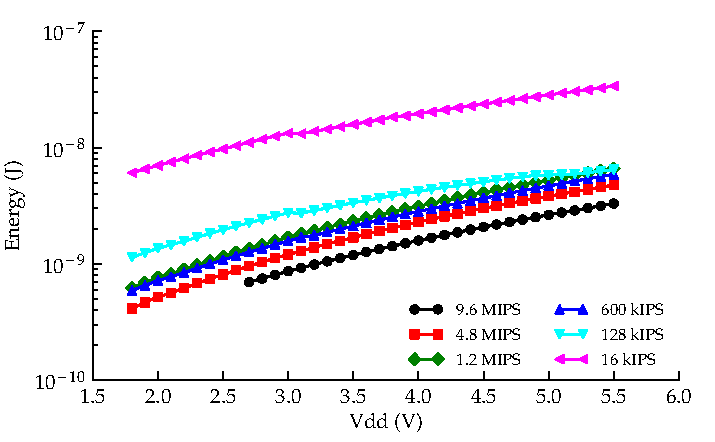
\includegraphics{content/appendices/microprocessorPowerMeasurements/graphics/Graph_ATtiny13V_Clock_JPI}
\par\end{centering}

\protect\caption{
\label{fig:ATtiny13VClkJPI}Energy consumed per instruction for the
Atmel ATtiny13V
}


\end{figure}



\subsubsection*{ATtiny25V}

\begin{sidewaystable}
\begin{centering}
\begin{tabular}{|r|r|r|r|r|r|r|r|r|}
\hline
Vdd  & 16 MHz  & 8 MHz  & 6.4 MHz  & 2 MHz  & 1 MHz  & 800 kHz  & 128 kHz  & 16 kHz \tabularnewline
\hline
1.80  & N/A  & N/A  & N/A  & 1.148E-03  & 4.106E-04  & 1.146E-03  & 7.622E-05  & 1.666E-04 \tabularnewline
1.90  & N/A  & N/A  & N/A  & 1.205E-03  & 4.319E-04  & 1.209E-03  & 7.858E-05  & 1.737E-04 \tabularnewline
2.00  & N/A  & N/A  & N/A  & 1.261E-03  & 4.531E-04  & 1.274E-03  & 8.121E-05  & 1.813E-04 \tabularnewline
2.10  & N/A  & N/A  & N/A  & 1.320E-03  & 4.754E-04  & 1.339E-03  & 8.464E-05  & 1.903E-04 \tabularnewline
2.20  & N/A  & N/A  & N/A  & 1.378E-03  & 4.984E-04  & 1.404E-03  & 8.981E-05  & 1.994E-04 \tabularnewline
2.30  & N/A  & N/A  & N/A  & 1.434E-03  & 5.195E-04  & 1.471E-03  & 9.486E-05  & 2.066E-04 \tabularnewline
2.40  & N/A  & N/A  & N/A  & 1.491E-03  & 5.413E-04  & 1.537E-03  & 9.642E-05  & 2.126E-04 \tabularnewline
2.50  & N/A  & N/A  & N/A  & 1.540E-03  & 5.671E-04  & 1.604E-03  & 9.903E-05  & 2.193E-04 \tabularnewline
2.60  & N/A  & N/A  & N/A  & 1.597E-03  & 5.912E-04  & 1.671E-03  & 1.008E-04  & 2.257E-04 \tabularnewline
2.70  & 6.283E-03  & 3.124E-03  & 1.765E-03  & 1.651E-03  & 6.163E-04  & 1.740E-03  & 1.030E-04  & 2.320E-04 \tabularnewline
2.80  & 6.551E-03  & 3.256E-03  & 1.842E-03  & 1.706E-03  & 6.425E-04  & 1.811E-03  & 1.053E-04  & 2.378E-04 \tabularnewline
2.90  & 6.826E-03  & 3.392E-03  & 1.916E-03  & 1.766E-03  & 6.683E-04  & 1.883E-03  & 1.072E-04  & 2.414E-04 \tabularnewline
3.00  & 7.097E-03  & 3.537E-03  & 1.995E-03  & 1.832E-03  & 6.963E-04  & 1.959E-03  & 1.094E-04  & 2.434E-04 \tabularnewline
3.10  & 7.380E-03  & 3.682E-03  & 2.081E-03  & 1.906E-03  & 7.284E-04  & 2.050E-03  & 1.118E-04  & 2.440E-04 \tabularnewline
3.20  & 7.695E-03  & 3.825E-03  & 2.172E-03  & 1.973E-03  & 7.623E-04  & 2.131E-03  & 1.143E-04  & 2.469E-04 \tabularnewline
3.30  & 7.996E-03  & 3.975E-03  & 2.253E-03  & 2.036E-03  & 7.925E-04  & 2.210E-03  & 1.170E-04  & 2.521E-04 \tabularnewline
3.40  & 8.288E-03  & 4.122E-03  & 2.340E-03  & 2.101E-03  & 8.216E-04  & 2.286E-03  & 1.190E-04  & 2.587E-04 \tabularnewline
3.50  & 8.605E-03  & 4.271E-03  & 2.425E-03  & 2.165E-03  & 8.516E-04  & 2.371E-03  & 1.208E-04  & 2.657E-04 \tabularnewline
3.60  & 8.915E-03  & 4.421E-03  & 2.510E-03  & 2.230E-03  & 8.824E-04  & 2.452E-03  & 1.222E-04  & 2.732E-04 \tabularnewline
\hline
\end{tabular}
\par\end{centering}

\protect\caption{Atmel ATtiny25V clocking current (Vdd 3.7V -- 5.5V)}


\end{sidewaystable}
\begin{sidewaystable}
\begin{centering}
\begin{tabular}{|r|r|r|r|r|r|r|r|r|}
\hline
Vdd  & 16 MHz  & 8 MHz  & 6.4 MHz  & 2 MHz  & 1 MHz  & 800 kHz  & 128 kHz  & 16 kHz \tabularnewline
\hline
3.70  & 9.232E-03  & 4.582E-03  & 2.599E-03  & 2.298E-03  & 9.122E-04  & 2.535E-03  & 1.235E-04  & 2.805E-04 \tabularnewline
3.80  & 9.550E-03  & 4.754E-03  & 2.687E-03  & 2.365E-03  & 9.436E-04  & 2.622E-03  & 1.246E-04  & 2.867E-04 \tabularnewline
3.90  & 9.908E-03  & 4.921E-03  & 2.776E-03  & 2.436E-03  & 9.746E-04  & 2.706E-03  & 1.258E-04  & 2.950E-04 \tabularnewline
4.00  & 1.025E-02  & 5.077E-03  & 2.864E-03  & 2.506E-03  & 1.006E-03  & 2.795E-03  & 1.269E-04  & 2.951E-04 \tabularnewline
4.10  & 1.057E-02  & 5.245E-03  & 2.962E-03  & 2.578E-03  & 1.040E-03  & 2.882E-03  & 1.280E-04  & 3.015E-04 \tabularnewline
4.20  & 1.092E-02  & 5.422E-03  & 3.054E-03  & 2.652E-03  & 1.074E-03  & 2.970E-03  & 1.278E-04  & 3.085E-04 \tabularnewline
4.30  & 1.128E-02  & 5.607E-03  & 3.153E-03  & 2.724E-03  & 1.108E-03  & 3.062E-03  & 1.279E-04  & 3.159E-04 \tabularnewline
4.40  & 1.161E-02  & 5.783E-03  & 3.250E-03  & 2.795E-03  & 1.143E-03  & 3.155E-03  & 1.270E-04  & 3.235E-04 \tabularnewline
4.50  & 1.198E-02  & 5.958E-03  & 3.348E-03  & 2.873E-03  & 1.177E-03  & 3.248E-03  & 1.266E-04  & 3.313E-04 \tabularnewline
4.60  & 1.235E-02  & 6.139E-03  & 3.445E-03  & 2.949E-03  & 1.210E-03  & 3.340E-03  & 1.254E-04  & 3.390E-04 \tabularnewline
4.70  & 1.272E-02  & 6.312E-03  & 3.549E-03  & 3.027E-03  & 1.248E-03  & 3.430E-03  & 1.240E-04  & 3.468E-04 \tabularnewline
4.80  & 1.311E-02  & 6.501E-03  & 3.653E-03  & 3.105E-03  & 1.284E-03  & 3.528E-03  & 1.230E-04  & 3.547E-04 \tabularnewline
4.90  & 1.349E-02  & 6.689E-03  & 3.757E-03  & 3.190E-03  & 1.319E-03  & 3.633E-03  & 1.229E-04  & 3.625E-04 \tabularnewline
5.00  & 1.387E-02  & 6.898E-03  & 3.860E-03  & 3.270E-03  & 1.358E-03  & 3.732E-03  & 1.237E-04  & 3.703E-04 \tabularnewline
5.10  & 1.427E-02  & 7.099E-03  & 3.965E-03  & 3.356E-03  & 1.396E-03  & 3.832E-03  & 1.248E-04  & 3.781E-04 \tabularnewline
5.20  & 1.464E-02  & 7.302E-03  & 4.075E-03  & 3.437E-03  & 1.432E-03  & 3.931E-03  & 1.262E-04  & 3.857E-04 \tabularnewline
5.30  & 1.506E-02  & 7.502E-03  & 4.181E-03  & 3.527E-03  & 1.471E-03  & 4.033E-03  & 1.277E-04  & 3.930E-04 \tabularnewline
5.40  & 1.547E-02  & 7.713E-03  & 4.297E-03  & 3.616E-03  & 1.512E-03  & 4.142E-03  & 1.293E-04  & 3.999E-04 \tabularnewline
5.50  & 1.588E-02  & 7.908E-03  & 4.415E-03  & 3.705E-03  & 1.552E-03  & 4.245E-03  & 1.311E-04  & 4.063E-04 \tabularnewline
\hline
\end{tabular}
\par\end{centering}

\protect\caption{Atmel ATtiny25V clocking current (VDD 3.7V -- 5.5V)}


\end{sidewaystable}
\begin{figure}
\begin{centering}
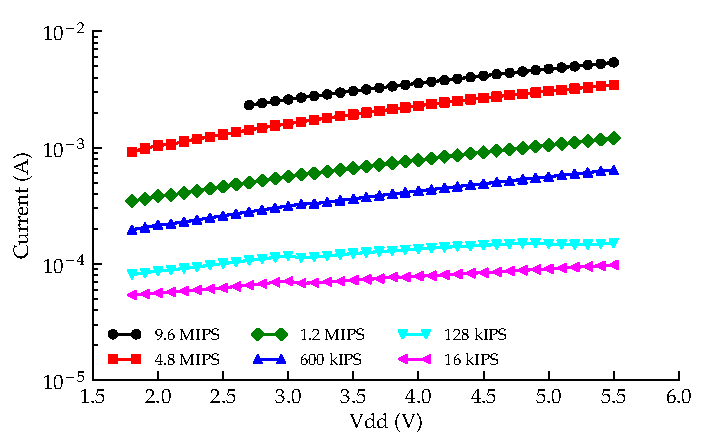
\includegraphics{content/appendices/microprocessorPowerMeasurements/graphics/Graph_ATtiny13V_Clock_Current}
\par\end{centering}

\protect\caption{\label{fig:ATtiny25VClkCurrent}Current consumption of the Atmel ATtiny25V
while clocking}


\end{figure}
\begin{figure}
\begin{centering}
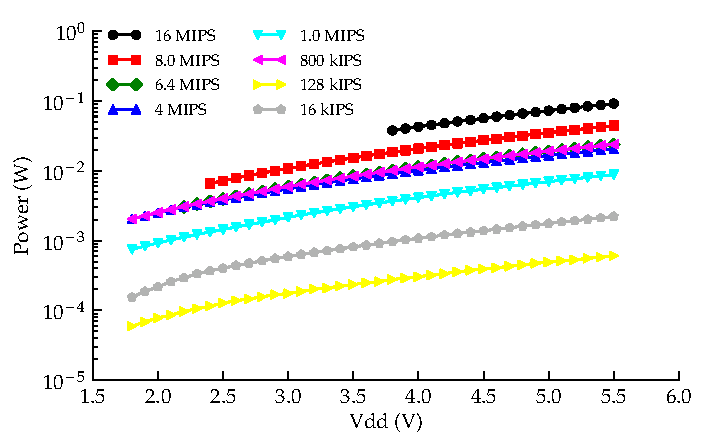
\includegraphics{content/appendices/microprocessorPowerMeasurements/graphics/Graph_ATtiny25V_Clock_Power}
\par\end{centering}

\protect\caption{
\label{fig:ATtiny25VClkPower}Power consumption of the Atmel ATtiny25V
while clocking
}


\end{figure}
\begin{figure}
\begin{centering}
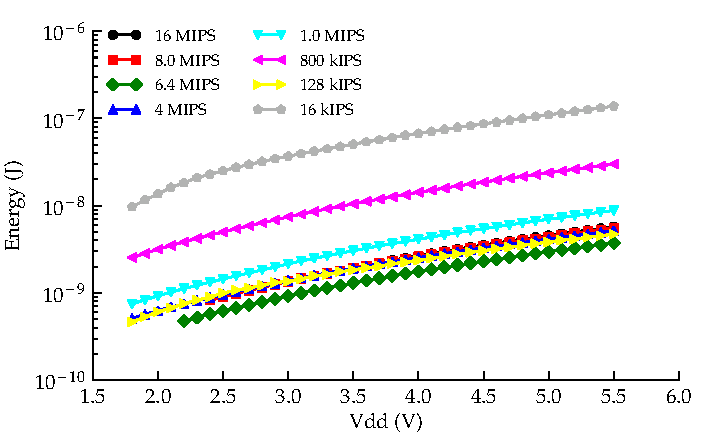
\includegraphics{content/appendices/microprocessorPowerMeasurements/graphics/Graph_ATtiny25V_Clock_JPI}
\par\end{centering}

\protect\caption{
\label{fig:ATtiny25VClkJPI}Energy consumed per instruction for the
Atmel ATtiny25V
}


\end{figure}



\subsubsection*{Microchip PIC16F1827}

\begin{sidewaystable}
\begin{centering}
\begin{tabular}{|r|r|r|r|r|r|r|r|r|}
\hline
Vdd  & 32 MHz  & 16 MHz  & 8 MHz  & 4 MHz  & 2 MHz  & 1 MHz  & 500 kHz  & 31 kHz \tabularnewline
\hline
1.80  & N/A  & 1.250E-03  & 8.043E-04  & 5.163E-04  & 3.912E-04  & 3.290E-04  & 1.327E-04  & 4.679E-06 \tabularnewline
1.90  & N/A  & 1.322E-03  & 8.483E-04  & 5.391E-04  & 4.066E-04  & 3.405E-04  & 1.367E-04  & 4.892E-06 \tabularnewline
2.00  & N/A  & 1.395E-03  & 8.930E-04  & 5.619E-04  & 4.220E-04  & 3.520E-04  & 1.402E-04  & 5.063E-06 \tabularnewline
2.10  & N/A  & 1.468E-03  & 9.382E-04  & 5.848E-04  & 4.375E-04  & 3.637E-04  & 1.436E-04  & 5.307E-06 \tabularnewline
2.20  & N/A  & 1.542E-03  & 9.841E-04  & 6.079E-04  & 4.528E-04  & 3.754E-04  & 1.471E-04  & 5.546E-06 \tabularnewline
2.30  & N/A  & 1.620E-03  & 1.031E-03  & 6.310E-04  & 4.683E-04  & 3.870E-04  & 1.503E-04  & 5.796E-06 \tabularnewline
2.40  & N/A  & 1.698E-03  & 1.078E-03  & 6.544E-04  & 4.838E-04  & 3.987E-04  & 1.535E-04  & 5.996E-06 \tabularnewline
2.50  & 2.711E-03  & 1.773E-03  & 1.126E-03  & 6.778E-04  & 4.996E-04  & 4.105E-04  & 1.567E-04  & 6.282E-06 \tabularnewline
2.60  & 2.826E-03  & 1.848E-03  & 1.172E-03  & 7.008E-04  & 5.150E-04  & 4.223E-04  & 1.599E-04  & 6.536E-06 \tabularnewline
2.70  & 2.939E-03  & 1.919E-03  & 1.214E-03  & 7.232E-04  & 5.301E-04  & 4.337E-04  & 1.631E-04  & 6.734E-06 \tabularnewline
2.80  & 3.050E-03  & 1.990E-03  & 1.255E-03  & 7.456E-04  & 5.450E-04  & 4.449E-04  & 1.662E-04  & 6.912E-06 \tabularnewline
2.90  & 3.163E-03  & 2.062E-03  & 1.297E-03  & 7.685E-04  & 5.605E-04  & 4.565E-04  & 1.695E-04  & 7.109E-06 \tabularnewline
3.00  & 3.277E-03  & 2.134E-03  & 1.338E-03  & 7.916E-04  & 5.758E-04  & 4.683E-04  & 1.728E-04  & 7.349E-06 \tabularnewline
3.10  & 3.391E-03  & 2.207E-03  & 1.380E-03  & 8.152E-04  & 5.917E-04  & 4.802E-04  & 1.763E-04  & 7.534E-06 \tabularnewline
3.20  & 3.507E-03  & 2.281E-03  & 1.422E-03  & 8.388E-04  & 6.074E-04  & 4.919E-04  & 1.797E-04  & 7.601E-06 \tabularnewline
3.30  & 3.623E-03  & 2.355E-03  & 1.465E-03  & 8.626E-04  & 6.235E-04  & 5.039E-04  & 1.829E-04  & 7.604E-06 \tabularnewline
3.40  & 3.445E-03  & 2.263E-03  & 1.438E-03  & 8.666E-04  & 6.386E-04  & 5.273E-04  & 1.940E-04  & 7.638E-06 \tabularnewline
3.50  & 3.445E-03  & 2.263E-03  & 1.439E-03  & 8.663E-04  & 6.390E-04  & 5.276E-04  & 1.942E-04  & 7.582E-06 \tabularnewline
3.60  & 3.447E-03  & 2.264E-03  & 1.439E-03  & 8.663E-04  & 6.389E-04  & 5.275E-04  & 1.943E-04  & 7.616E-06 \tabularnewline
\hline
\end{tabular}
\par\end{centering}

\protect\caption{Microchip PIC16F1827 clocking current (Vdd 0V -- 3.6V)}


\end{sidewaystable}
\begin{sidewaystable}
\begin{centering}
\begin{tabular}{|r|r|r|r|r|r|r|r|r|}
\hline
Vdd  & 32 MHz  & 16 MHz  & 8 MHz  & 4 MHz  & 2 MHz  & 1 MHz  & 500 kHz  & 31 kHz \tabularnewline
\hline
3.70  & 3.449E-03  & 2.265E-03  & 1.439E-03  & 8.663E-04  & 6.392E-04  & 5.277E-04  & 1.945E-04  & 7.617E-06 \tabularnewline
3.80  & 3.449E-03  & 2.265E-03  & 1.440E-03  & 8.665E-04  & 6.393E-04  & 5.279E-04  & 1.947E-04  & 7.649E-06 \tabularnewline
3.90  & 3.450E-03  & 2.265E-03  & 1.440E-03  & 8.667E-04  & 6.397E-04  & 5.283E-04  & 1.950E-04  & 7.603E-06 \tabularnewline
4.00  & 3.451E-03  & 2.267E-03  & 1.441E-03  & 8.669E-04  & 6.396E-04  & 5.283E-04  & 1.952E-04  & 7.634E-06 \tabularnewline
4.10  & 3.452E-03  & 2.267E-03  & 1.441E-03  & 8.672E-04  & 6.401E-04  & 5.286E-04  & 1.955E-04  & 7.633E-06 \tabularnewline
4.20  & 3.453E-03  & 2.268E-03  & 1.442E-03  & 8.673E-04  & 6.401E-04  & 5.286E-04  & 1.957E-04  & 7.667E-06 \tabularnewline
4.30  & 3.454E-03  & 2.269E-03  & 1.442E-03  & 8.675E-04  & 6.404E-04  & 5.290E-04  & 1.960E-04  & 7.620E-06 \tabularnewline
4.40  & 3.454E-03  & 2.269E-03  & 1.443E-03  & 8.679E-04  & 6.405E-04  & 5.293E-04  & 1.961E-04  & 7.660E-06 \tabularnewline
4.50  & 3.456E-03  & 2.270E-03  & 1.443E-03  & 8.681E-04  & 6.410E-04  & 5.294E-04  & 1.964E-04  & 7.663E-06 \tabularnewline
4.60  & 3.457E-03  & 2.271E-03  & 1.444E-03  & 8.684E-04  & 6.412E-04  & 5.297E-04  & 1.966E-04  & 7.704E-06 \tabularnewline
4.70  & 3.458E-03  & 2.271E-03  & 1.444E-03  & 8.687E-04  & 6.416E-04  & 5.300E-04  & 1.969E-04  & 7.664E-06 \tabularnewline
4.80  & 3.458E-03  & 2.272E-03  & 1.445E-03  & 8.690E-04  & 6.417E-04  & 5.303E-04  & 1.972E-04  & 7.710E-06 \tabularnewline
4.90  & 3.460E-03  & 2.273E-03  & 1.446E-03  & 8.692E-04  & 6.421E-04  & 5.307E-04  & 1.976E-04  & 7.721E-06 \tabularnewline
5.00  & 3.461E-03  & 2.274E-03  & 1.446E-03  & 8.695E-04  & 6.424E-04  & 5.310E-04  & 1.979E-04  & 7.757E-06 \tabularnewline
5.10  & 3.463E-03  & 2.275E-03  & 1.447E-03  & 8.697E-04  & 6.428E-04  & 5.314E-04  & 1.983E-04  & 7.733E-06 \tabularnewline
5.20  & 3.464E-03  & 2.276E-03  & 1.448E-03  & 8.699E-04  & 6.433E-04  & 5.319E-04  & 1.986E-04  & 7.762E-06 \tabularnewline
5.30  & 3.465E-03  & 2.277E-03  & 1.448E-03  & 8.703E-04  & 6.437E-04  & 5.326E-04  & 1.991E-04  & 7.797E-06 \tabularnewline
5.40  & 3.467E-03  & 2.278E-03  & 1.449E-03  & 8.708E-04  & 6.444E-04  & 5.332E-04  & 1.996E-04  & 7.777E-06 \tabularnewline
5.50  & 3.468E-03  & 2.279E-03  & 1.450E-03  & 8.711E-04  & 6.449E-04  & 5.336E-04  & 2.002E-04  & 7.833E-06 \tabularnewline
\hline
\end{tabular}
\par\end{centering}

\protect\caption{Microchip PIC16F1827 clocking current (Vdd 3.7V -- 5.5V)}
\end{sidewaystable}
\begin{figure}
\begin{centering}
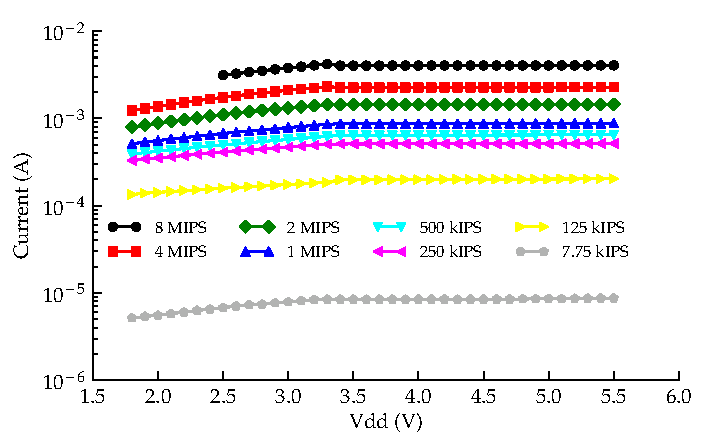
\includegraphics{content/appendices/microprocessorPowerMeasurements/graphics/Graph_PIC16F1827_Clock_Current}
\par\end{centering}

\protect\caption{\label{fig:16F1827ClkCurrent}Current consumption of the Microchip
PIC16F1827 while clocking}


\end{figure}
\begin{figure}
\begin{centering}
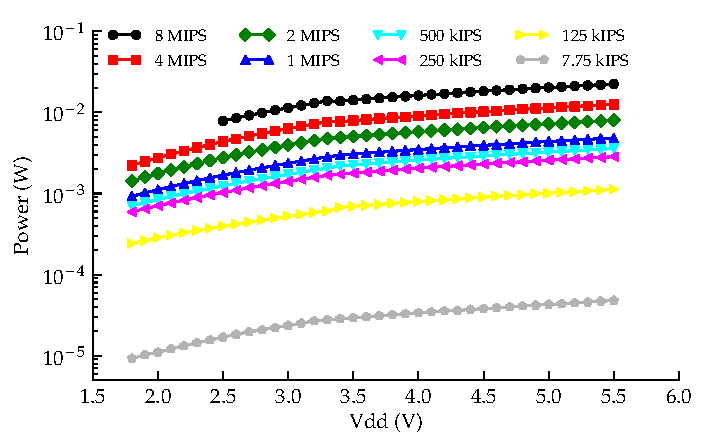
\includegraphics{content/appendices/microprocessorPowerMeasurements/graphics/Graph_PIC16F1827_Clock_Power}
\par\end{centering}

\protect\caption{
\label{fig:16F1827ClkPower}Power consumption of the Microchip PIC16F1827
while clocking
}


\end{figure}
\begin{figure}
\begin{centering}
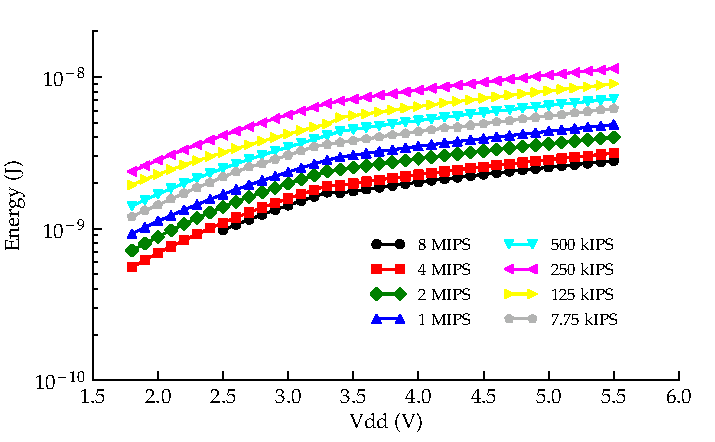
\includegraphics{content/appendices/microprocessorPowerMeasurements/graphics/Graph_PIC16F1827_Clock_JPI}
\par\end{centering}

\protect\caption{
\label{fig:16F1827ClkJPI}Energy consumed per instruction for the
Microchip PIC16F1827
}


\end{figure}



\section{Microprocessor Test Code}


\subsection{ATMEL ATtiny13V and ATtiny25}

Code was written in AVRStudio 4.18 (build 684) and compiled using
WinAVR (AVR-GCC compiler for windows available from \url{http://winavr.sourceforge.net/}.
Chip programming was done using an Atmel AVR STK500 demonstration
board with serial interface.


\subsubsection*{Sleep}

Programming fuses were all disabled (Watchdog, brown-out detect, clock
divider) and clock selection was set to `Int. RC Osc 128kHz; Start-up
time; 14 CK + 0ms'

\lstinputlisting[caption={ATtiny25V Sleep Proceedure},label={code:ATtiny25VSleepCode}]{content/appendices/microprocessorPowerMeasurements/code/ATtiny13V_sleep.c}


\subsubsection*{Clocking}

\lstinputlisting[caption={ATtiny25V Clocking Proceedure},label={code:ATtiny25VClockingCode}]{content/appendices/microprocessorPowerMeasurements/code/ATtiny13V_clocking.c}


\subsection{Microchip 12F675}

Code was written in MPLAB v8.6 in C and compiled using HI-TECH C v9.60.
Chip programming was done using PICkit 2 Programmer software v2.61.
\footnote{Downloading to the 12F675s with MPLAB led to corruption of the internal
oscillators, causing them fail.%
}


\subsubsection*{Sleep}


\subsection{Microchip 16F1827}

Code written in MPLAB v8.6 in C and compiled using HI-TECH C v 9.60.
Chip programming was done using PICkit 2 Programmer software v2.61,
however in order to program the 16F1827 with the PICkit 2 programmer
a patch was applied to the device file list. This patch was retrieved
from \url{http://www.uploadarchief.net/files/download/pk2patch16x.zip}
on the 12th May 2011.


\subsubsection*{Sleep}

The specified sleep current of 30nA was not achievable. In an attempt
to reach the specified current, the program was written in assembler.
The assembler version of the code was used in the measurement data.
The assembler version gave a lower sleep current than the C version,
probably not as a result of the compiler but as due to a more thorough
initialisation routine.

\lstinputlisting[caption={16F1827 Sleep Proceedure - HI-TECH C version},label={code:PIC16F1827SleepCodeC}]{content/appendices/microprocessorPowerMeasurements/code/PIC16F1827_sleep.c}

\lstinputlisting[caption={16F1827 Sleep Proceedure - MPASM assembler version},label={code:PIC16F1827SleepCodeASM}]{content/appendices/microprocessorPowerMeasurements/code/PIC16F1827_sleep.asm}


\subsubsection*{Clocking}

\lstinputlisting[caption={PIC16F1827 Clocking Proceedure},label={code:PIC16F1827ClockingCode}]{content/appendices/microprocessorPowerMeasurements/code/PIC16F1827_clocking.c}


\subsection{Freescale M9S08QG8}

Code was written using Freescale's bundled IDE, CodeWarrior v5.90,
and downloaded using a supplied USB demo board (DEMO9S08QG8E).


\subsubsection*{Sleep}

\lstinputlisting[caption={M9S08QG8 Sleep Proceedure},label={code:M9S08QG8ClockingCode}]{content/appendices/microprocessorPowerMeasurements/code/MC9S08QG8_sleep.c}
